\ifx\bookMode\undefined
\documentclass[12pt]{article}
\usepackage{373,graphicx,placeins}
\fi

\newcommand{\figurescale}{0.8}

\BeginDocument

\HWNum{CS373 - Spring 2012}{0}{Thursday April 5 at 2:00 PM in class (151 Everitt Lab)}
\Title{Problem Set 4}
\MakeTitleHW

%\hline

Please \underline{follow} the homework format guidelines posted on the class web
page:

\centerline{\url{\CourseWebpage}}
%\hline
\bigskip

\begin{enumerate}

%Problem 1
    \item \ProblemTtl{CFG Parsing}{Comprehension}{15}
    
    RNA molecules are crucial to all life on Earth.  In fact, they're so important, some researchers theorize these molecules may have been the start of all life on Earth\footnote{http://en.wikipedia.org/wiki/RNA\_world\_hypothesis}.  For our purposes, RNAs are represented as strings on the alphabet $\Sigma=\{a,u,c,g\}$.  The following grammar comes from an actual research paper\footnote{http://www.biomedcentral.com/1471-2105/5/71} about computational analysis of RNA:
    
    $S \rightarrow LS \;|\; L$
    
    $L \rightarrow aFu \;|\; uFa \;|\; cFg \;|\; gFc \;|\; a \;|\; u \;|\; c \;|\; g$
    
    $F \rightarrow aFu \;|\; uFa \;|\; cFg \;|\; gFc \;|\; LS$
    
    \begin{enumerate}
    	\item Put this grammar in CNF (3 points)
    	\item Provide the CYK table for these strings: 
   	\begin{itemize}
    		\item $w_1=gaccuc$ (4 points)
		\item $w_2=uggu$ (3 points)
   	 \end{itemize}
    	\item Prove that the language accepted by this grammar is actually regular. (3 points)
	\item Can you explain why these researchers are interested in parsing a regular language with a CFG?  (Hint: Think about part b and look at Figure 1 in the paper.) (2 points)
    \end{enumerate}
    
%Problem 2
    \item \ProblemTtl{Non-Context-Free Languages}{Proof}{10}
     
     Provide \emph{two} proofs that the following languages are not context-free.  First, provide a proof using the the pumping lemma for CFLs.  Second, provide a proof using closure properties of CFLs.  You may assume that the languages Sipser used when demonstrating the pumping lemma (see Sipser Examples 2.36, 2.37, and 2.38 pp. 126) are known to be non-context-free.
    \begin{enumerate}
  	\item $\{ 0^n 1^{2m} 0^{m+k} \;|\; 0 \le n \le m, k \ge 0 \}$
	\item $\{w\in \{a,b,c\}^* \;|\; \#a(w)=\#b(w)=\#c(w)\}$
    \end{enumerate}
    
%Problem 3
\item \ProblemTtl{The Chomsky Hierarchy}{Proof}{15}
	
	In class, we've covered several classes in the Chomsky Hierarchy: regular, context-free, and context-sensitive languages:

	 \begin{center}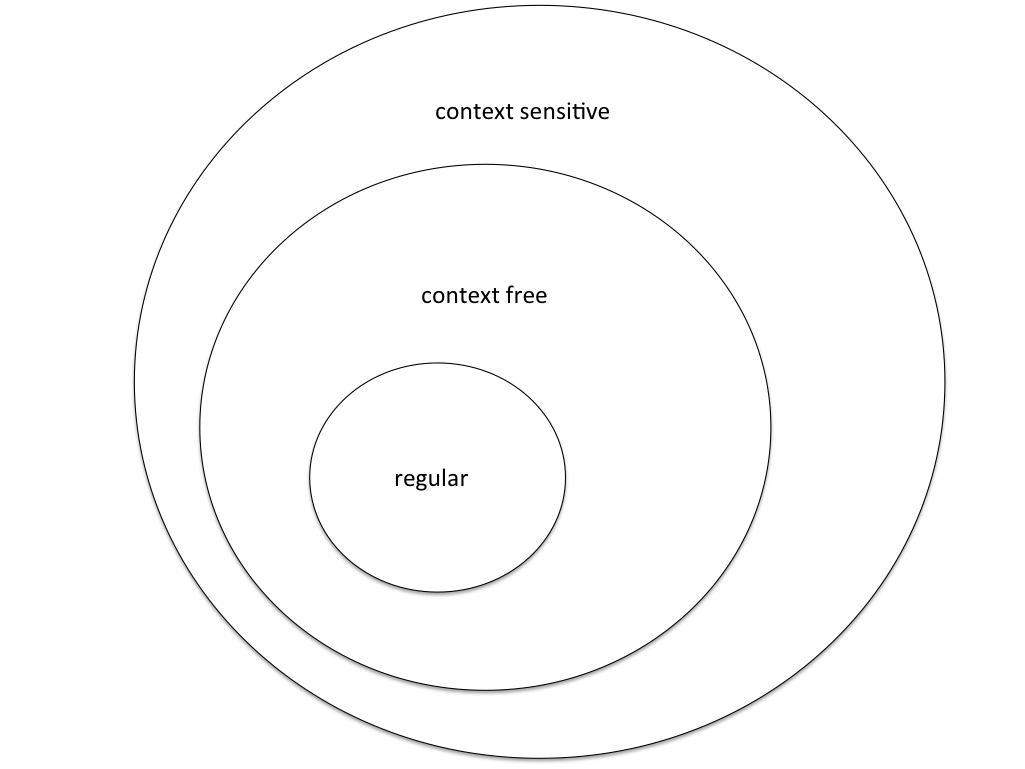
\includegraphics[scale=.25]{diagram/Slide1.png}\end{center}
	
	Based on what you've learned, it should be possible to assign languages from these classes to their most exclusive (or least general) class in the Chomsky Hierarchy.  For example, we know the language $L=\{0^n1^n | n\ge0\}$ is context-free, but not regular.  We used the pumping lemma for regular languages to prove that it is not regular (see Sipser, Example 1.73, pp. 80) and wrote a CFG to prove that it is context-free (see Sipser, Section 2.1, pp. 100).  It fits into the hierarchy in the region shaded below:
	
	 \begin{center}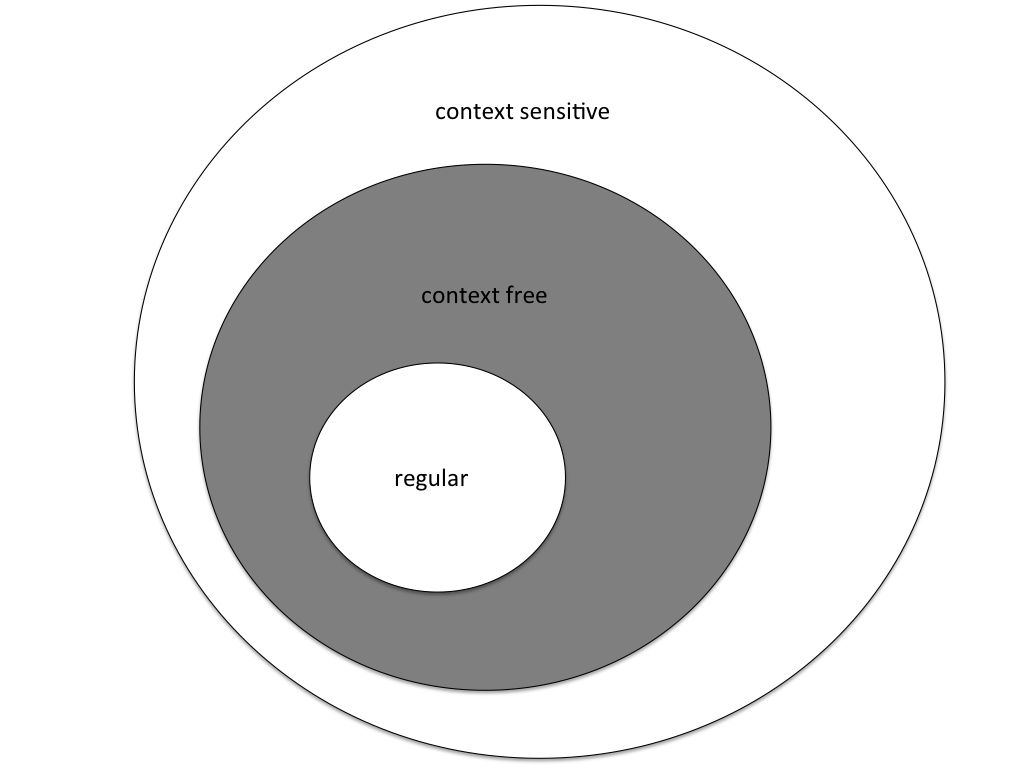
\includegraphics[scale=.25]{diagram/Slide2.png}\end{center}
	
	Using all your knowledge of formal languages, place these languages into the most exclusive class in the hierarchy you know.  State the class, and provide a proof that it is a member of that class.  Also provide a proof that it is not a member of a more exclusive class.  None of these languages belong exclusively to classes we haven't yet covered, and all of the languages are on the alphabet $\Sigma=\{0,1\}$.
	\begin{enumerate}
	\item $\{w \;|\; \#0(w)=\#1(w)\}$ (5 points)
    	\item $\{w \;|\; w=w^r, \#0(w)=\#1(w)\}$ (5 points)
	\item $\{w=xy \;|\; x,y\in\Sigma^* \text{ and } \#0(x)+\#1(x)=\#0(y)+\#1(y)\}$ (5 points)
	\end{enumerate}
%Problem 4
    \item \ProblemTtl{Closure Properties of CFLs}{Proof}{25}
    
    	 As on the midterm, the shuffle operation combines two strings $x$ and $y$ in all possible ways that preserve the original order of symbols from $x$ and $y$.  For example, if $x=x_1x_2x_3$ and $y=y_1y_2y_3y_4$, some valid shufflings are $y_1x_1y_2x_2x_3y_3y_4$ and $x_1x_2y_1y_2y_3x_3y_4$.  We define the shuffle of two languages $shuffle(A,B)$ to be the shuffling of all the words in $A$ with all the words in $B$.  More explicitly,
	\begin{center} $shuffle(A,B)=\bigcup\limits_{x \in A}\bigcup\limits_{y \in B} shuffle(x,y)$ \end{center}
	\begin{enumerate}
	\item Prove that, if $A$ is context-free and $B$ is regular, $shuffle(A,B)$ is context-free. (8 points)
	\item Prove that, if $A$ and $B$ are context-free, $shuffle(A,B)$ is not necessarily context-free. (8 points)
	\item For a binary language $L$ over $\Sigma=\{0,1\}$, we define the function $p$ (which maps a single string to a set of strings) as follows:
	
	\begin{center}$p(w) = \{ x \in \{0,1\}^* \;|\; \#0(w) = \#0(x), \#1(w) = \#1(x) \}$\end{center}
	
	Using $p$, we define the operation $p$ on languages:
	
	\begin{center}$p(L) = \bigcup\limits_{w \in L} p(w)$\end{center} 
	
	Let $L$ be a regular language.  Show that $p(L)$ is context-free. (9 points)
    \end{enumerate}
    
%Problem 5
    \item \ProblemTtl{Context Sensitive Grammars}{Design}{20}
    
    Give a context sensitive grammar for the language:
    \begin{center}$A = \{0^k \;|\; k = 2^i+1,i\ge0\}$\end{center}
    
%Problem 6
    \item \ProblemTtl{Turing Machines}{Design}{15}
    
    Give a "higher level" (see "Examples of Turing machines", Sipser pp. 142) description of a Turing machine for the language:
    
    \begin{center}$A=\{a^ib^jc^k | i\%j=k \text{ and } i,j,k\ge1\}$\end{center}
    
    Where $\%$ is the \href{http://en.wikipedia.org/wiki/Modulo_operation}{modulo operator}.
    
\end{enumerate}
\EndDocument
